% WM-Concord capstone report, Fall 2026, Group 6
% Adapted from the course template (originally by faculty at Reykjavik University, Iceland)

\documentclass[11pt]{scrartcl}

% Adapted from an original template by Hlyni Arnórssyni, Reykjavik University, Iceland
%
% ------------------------------ SETTINGS
\usepackage{geometry}

\geometry{
	paper=a4paper, % Paper size
	top=2.5cm, % Top margin
	bottom=2.5cm, % Bottom margin
	left=2.5cm, % Left margin
	right=2.4cm, % Right margin
	headheight=0.75cm, % Header height
	footskip=1.5cm, % Space from the bottom margin to the baseline of the footer
	headsep=0.75cm, % Space from the top margin to the baseline of the header
	%showframe, % Uncomment to show how the type block is set on the page
}

\usepackage{blindtext}
%-------------------------------- Character encoding ----------------------------
\usepackage[T1]{fontenc}
\usepackage[utf8]{inputenc}

%----------------------------- Mathematics packages from AMS ---------------

\usepackage{amsmath, amsfonts, amsthm, amssymb}
\usepackage{braket, nicefrac}

% ----------- International System of Units
\usepackage{siunitx}

%------------------------------ Lists / numbers -------------------------
\usepackage{enumitem, multicol}

%------------------------------- Figure insertions --------------
\usepackage{graphicx, float}  % Use option [H] to force the placement of a figure
\usepackage{keystroke}
\usepackage{pgfplots}\usepgfplotslibrary{units}\pgfplotsset{compat=1.16}




%%%%%%%%%%%%%%%%%%%%%%%%%% Hyperlink References %%%%%%%%%%%%%%%%%%%%%%%%%%%
\usepackage{hyperref}

%--------------------% Storage Path for images %-----------------%
\graphicspath{{graphics/}{Graphics/}{./}}
\usepackage{lmodern}          % sharp vector fonts in the PDF
\usepackage{graphicx,epsfig}
\usepackage{xcolor}
\usepackage{booktabs}
\usepackage{array}
\hypersetup{
   colorlinks   = true,
   urlcolor     = blue,
   linkcolor    = blue,
   citecolor    = red,
   setpagesize  = false,
   linktocpage  = true,
}
\graphicspath{ {fig/} }
\addtokomafont{disposition}{\rmfamily}   % section titles in the same font as the text

\renewenvironment{abstract}{
    \centering
    \textbf{Abstract}
    \vspace{0.4cm}
    \par\itshape
    \begin{minipage}{0.8\linewidth}}{\end{minipage}
    \noindent\ignorespaces
}
% ------------------------------------------------------------------------------------------------------------------------

\begin{document}
\begin{titlepage}
	\centering
	
\includegraphics[width=0.45\textwidth]{GW_logo.eps}\par
	\vspace{1.5cm}
	{\scshape\LARGE Data Science Program \par}
	\vspace{0.8cm}
	{\scshape\Large Capstone Report, Fall 2026\par}
	\vspace{1.5cm}
	{\huge\bfseries WM-Concord: Do World Model Diagnostics Agree?\par}
	\vspace{0.4cm}
	{\Large A Cross Diagnostic Validity Study of World Model Diagnostics\par}
	\vspace{1.5cm}
	{\Large\itshape Venkatesh Nagarjuna \\ Siddardha Reddy \\ Nikhil Obuleni \\ Viharika Vemparala\par}
	\vspace{1cm}
	supervised by\par
	Amir Jafari
	\vfill
	\begin{abstract}
	    Sequence models are often said to learn a ``world model'': an internal picture of the state of the
	    domain they were trained on. The literature tests this claim with four families of diagnostics:
	    next token validity, state equivalence metrics based on the Myhill Nerode theorem, inductive bias
	    probes, and representation probing. These diagnostics have never been run on the same models, and on
	    Othello they already reach opposite conclusions. WM-Concord runs all four diagnostics on one
	    controlled zoo of small sequence models trained on domains with a known ground truth automaton
	    (Othello now; navigation and a held out program interpreter next). We ask whether the diagnostics
	    rank models the same way, why they disagree when they do, and which one best predicts failure on
	    related but shifted tasks. On 81 Othello models, under a preregistered analysis, the four diagnostics
	    agree strongly (Kendall W 0.87), but almost all of that agreement is shared competence: with the
	    validation legal move rate controlled, the agreement falls to W 0.27 and no pair among the three
	    diagnostics that can be separated from competence still agrees. The remaining disagreement is not
	    explained by architecture, scale or training data. Only the representation probe adds to the legal
	    move rate in predicting fragility, and an exploratory check shows that this signal comes from
	    differences between training distributions, not from comparable models.
	\end{abstract}
	\vfill
	{\small George Washington University, Washington DC \quad\textbullet\quad \today\par}
\end{titlepage}

\tableofcontents
\newpage

% ------------------------------------------------------------------------------------------------------------------------
\section{Introduction}

Whether a sequence model trained only to predict the next token builds a coherent internal model of its
domain is one of the central open questions in current machine learning. Several research groups have built
diagnostics to answer it, but each group uses its own instrument, on its own models, in its own domain. The
same Othello models have been reported both as having a world model~\cite{li2023othello, yuan2025revisiting}
and as lacking a coherent one~\cite{vafa2024evaluating, vafa2025inductive}. This project does not propose a
new diagnostic. It measures whether the existing ones agree, and which one can be trusted.

\paragraph{Contributions.}
\begin{itemize}
    \item The first head to head comparison of four world model diagnostics on the same models and the same
    ground truth.
    \item A test of which diagnostic predicts failure on related but shifted tasks, judged against a
    fragility suite that is frozen before any diagnostic is run.
    \item An open source benchmark (WM-Concord) with one common interface, so a future diagnostic can be
    compared against these four on identical ground truth.
\end{itemize}

\paragraph{What we found so far.} On the first domain, Othello, we trained 81 models (three architectures,
three scales, three training distributions, three seeds), all of which passed a preregistered admission rule,
and scored every one with all four diagnostics and two versions of a fragility suite. The diagnostics agree on
which models are better, but they agree because all of them follow competence, the model's legal move rate:
once competence is controlled for, the agreement largely disappears (Section~\ref{sec:h1}). Where they
disagree, the disagreement is consistent with seed noise (Section~\ref{sec:h2}). No diagnostic is a reliable
predictor of fragility: the representation probe adds to the legal move rate under the preregistered test,
but an exploratory analysis traces this to the models trained on human games, which are both the most fragile
and the least probe readable (Section~\ref{sec:h3}). The practical message for anyone using these tools is to
report several diagnostics, always with a competence control, rather than trust any single one.

% ------------------------------------------------------------------------------------------------------------------------
\section{Problem Statement}

The four diagnostic families studied in this project are:
\begin{description}
    \item[D1, next token validity.] The fraction of the model's proposed next tokens that are legal in the
    true state.
    \item[D2, state equivalence.] Compression error (two histories that reach the same state are treated
    differently) and distinction error (two different states are treated the same), following
    \cite{vafa2024evaluating}.
    \item[D3, inductive bias probes.] How the model adapts to small synthetic tasks generated from the true
    world model~\cite{vafa2025inductive}.
    \item[D4, representation probing.] Whether the true state can be read from the model's internal
    activations by a probe, checked against a control task and by causal intervention~\cite{li2023othello}.
\end{description}

We test four hypotheses:
\begin{description}
    \item[H1, concordance.] Do the four diagnostics rank the same models in the same order?
    \item[H2, disagreement.] When they disagree, is the disagreement systematic (tied to architecture,
    scale, or training data) or just noise?
    \item[H3, predictive validity.] Which diagnostic best predicts failure on a frozen suite of related but
    shifted tasks?
    \item[H4, generalization.] Do the answers hold on a held out domain?
\end{description}

\paragraph{Challenges.} The diagnostics measure different things (behaviour, adaptation, and internal
activations), so their scores are not on a common scale; we therefore compare only rankings. The state
equivalence metrics cannot be computed exactly in large domains and must be estimated by sampling. Probes can
report structure the model does not actually use. And every diagnostic is likely to reward a better trained
model, so agreement can come from competence alone. The design handles each of these in
Section~\ref{sec:method}.

% ------------------------------------------------------------------------------------------------------------------------
\section{Related Work}
\label{sec:related}

% Instructor Review 2: at least 10 works, each summarised in our own words, each stating how WM-Concord
% differs. Every cited work goes in references.bib. Draft due October 6, complete by October 20.
%
% Done (12): li2023othello, yuan2025revisiting, nanda2023emergent, toshniwal2022chess,
%   vafa2024evaluating, vafa2025inductive, hewitt2019control, belinkov2022probing,
%   jacobs2021measurement, raji2021benchmark, and (Review 5) cameron2008bootstrap,
%   bouthillier2021variance. All are in references.bib.

\subsection{Representation probing}

Li et al.~\cite{li2023othello} trained a GPT model on Othello move sequences only. The model never sees a
board or the rules, yet it proposes legal moves almost every time, and probes trained on its internal
activations recover the board state. They then edited the decoded board inside the model and showed that
its next move predictions changed to match, which is evidence that the representation is used and not only
present. Yuan and S{\o}gaard~\cite{yuan2025revisiting} extended this to seven language models fine tuned on
Othello and found similar board representations across all of them, which they read as support for a real
world model. Both works use probing as the only instrument. WM-Concord uses probing as one of four
diagnostics, adds a control task and a causal check, and compares its verdict with the other three on the
same models.

Nanda et al.~\cite{nanda2023emergent} returned to the same Othello model and showed that the board is in
fact linearly represented, but relative to the player whose turn it is (``mine'' and ``theirs'') rather than
in absolute colours. With these labels a single linear layer reads the board almost perfectly, and adding or
subtracting a probe direction inside the model flips its view of a square and changes its next move
predictions accordingly. Our reproduction gate uses this result: our linear probes match their published
accuracies within one percentage point on five of six values. WM-Concord takes their mine and theirs labels
as the default for diagnostic D4, and asks whether a model that passes this probe also passes the three
diagnostics that do not look inside the model.

Toshniwal et al.~\cite{toshniwal2022chess} used chess as a testbed for state tracking in language models.
They trained transformers on games written as move sequences and tested state tracking with prompts that ask
for the starting or ending square of a piece at a given point in the game, so the board is read from the
model's own predictions rather than from its activations. They found that state tracking improves with more
training data and when some training positions include the type of the piece that moved. Their evaluation is
a behavioural one, close in spirit to next token validity. WM-Concord keeps such behavioural tests (D1) and
places them next to internal (D4) and structural (D2, D3) tests on the same models.

\subsection{State equivalence metrics}

Vafa et al.~\cite{vafa2024evaluating} define the domain as a deterministic finite automaton and derive two
metrics from the Myhill Nerode theorem. Compression error measures whether the model gives the same
continuations to two histories that end in the same state; distinction error measures whether it can tell
apart histories that end in different states. On taxi routes in Manhattan, Othello, and logic puzzles, models
that looked good on next token accuracy failed these metrics, and a map reconstructed from the navigation
model contained streets that do not exist. Models trained on random walks built more coherent world models
than models trained on shortest paths. That work compares its metrics only with next token accuracy.
WM-Concord uses them as diagnostic D2, adopts their three training distributions, and compares them with all
three other diagnostics and with an external fragility criterion.

\subsection{Inductive bias probes}

Vafa et al.~\cite{vafa2025inductive} ask a different question: does a model's inductive bias point at the
true world model? They adapt a pretrained model to small synthetic datasets generated from a postulated world
model and test whether it extrapolates the way that world model would. A model trained on orbital
trajectories predicted them well, but symbolic regression on the adapted model recovered force laws that make
no physical sense. This is our diagnostic D3. WM-Concord applies it to the same zoo as the other diagnostics,
so its verdict can be compared model by model.

\subsection{Probing confounds}

Hewitt and Liang~\cite{hewitt2019control} pointed out that a high probe accuracy does not show that the
model encodes a property, because an expressive probe can learn the task by itself. They proposed control
tasks: the same inputs with labels assigned at random to each input type, so the labels carry no structure
from the model. Selectivity, the probe's accuracy on the real task minus its accuracy on the control task,
measures how much of the accuracy comes from the model rather than from the probe. They found that larger
probes, such as multilayer perceptrons, often reach high accuracy with low selectivity. WM-Concord reports
selectivity, not raw accuracy, for every D4 probe, using their control task construction, and adds a layer 0
baseline because the token embedding alone already reads part of the Othello board.

Belinkov~\cite{belinkov2022probing} reviewed the probing classifier method and its limits. A probe shows that
information can be decoded from a representation, not that the model uses it; results depend on the choice of
probe and on the baseline it is compared with; and the correlation between probe accuracy and model behaviour
is not a causal link. The review points to controls, simpler probes, and interventions on the representation
as ways to close these gaps. WM-Concord follows this advice for D4 with a control task, a linear probe as the
default, and a causal check, and records models whose state is decodable but not used as a separate outcome.

\subsection{Measurement validity in ML evaluation}

Jacobs and Wallach~\cite{jacobs2021measurement} brought measurement modelling from the social sciences to
computational systems. An unobservable theoretical construct, such as fairness, is only ever measured through
an operationalization, and every operationalization makes assumptions that must be checked. They describe how
to do so through reliability and several kinds of validity, including convergent validity (do different
measures of the same construct agree?) and predictive validity (does the measure predict outcomes it should
predict?). WM-Concord treats ``world model'' as such a construct and the four diagnostics as its competing
operationalizations: H1 and H2 test their convergent validity, and H3 tests their predictive validity against
the fragility suite.

Raji et al.~\cite{raji2021benchmark} argued that popular machine learning benchmarks are often presented as
measures of general ability while they test narrow, specific tasks, so a high score is read as evidence for a
broad capability that the benchmark cannot establish. They call for benchmarks to state clearly what they
measure and to be validated against that claim. World model diagnostics face the same risk: each paper takes
a pass on its own diagnostic as evidence that the model has a world model. WM-Concord asks whether these
diagnostics measure the same thing at all, and which of them is backed by an external outcome.

\subsection{Inference when runs are not independent}

Cameron, Gelbach and Miller~\cite{cameron2008bootstrap} studied regression inference when observations come in
groups that share unobserved influences, such as workers in the same state. Standard errors that treat every
observation as independent are then too small, and the problem is worst when there are few groups. They show
that bootstrap methods which resample whole groups give much more honest tests, and that some refinements of
them stay reliable even when there are few groups. Bouthillier et al.~\cite{bouthillier2021variance}
measured how much the results of machine learning benchmarks move when only the random seed, the data order
or the initialisation changes, and found that this variation is often as large as the differences papers
report between methods; they recommend running several seeds and building that variation into every
comparison. WM-Concord trains three seeds of every configuration, so its 81 Othello models form 27 groups of
near copies. Following both works, every interval in this report resamples whole configurations, and H2 judges
disagreement against the spread between seeds of the same configuration.

\subsection{How WM-Concord differs}

These papers reach opposite conclusions about the same domain, but they use different instruments on
different models, so their disagreement cannot be interpreted. WM-Concord runs all four instruments on one
shared zoo of models with a known ground truth, which turns the disagreement into something that can be
measured (H1, H2) and judged against an external criterion (H3).

% ------------------------------------------------------------------------------------------------------------------------
\section{Data and Domains}
\label{sec:data}

All domains are defined by a deterministic finite automaton (DFA), so the true state is known at every step.
Every domain emits the same triple: token sequence, true state, and the set of legal next tokens.

\begin{table}[H]
    \centering
    \small
    \begin{tabular}{>{\raggedright\arraybackslash}p{3.2cm}>{\raggedright\arraybackslash}p{4.2cm}>{\raggedright\arraybackslash}p{6.6cm}}
    \toprule
    Domain & State & Training distributions \\
    \midrule
    Othello (done) & board position and player to move & synthetic, championship, mixed \\
    Navigation (next) & current intersection on a street graph & shortest paths, noisy shortest paths, random walks \\
    Interpreter (held out) & registers and stack of a small machine & random, short structured, long structured \\
    \bottomrule
    \end{tabular}
    \caption{The three domains. Othello is complete; navigation and the interpreter follow the same pipeline.}
    \label{tab:domains}
\end{table}

\subsection{Othello}
The Othello state consists of the $8\times8$ board together with the player to move. Following the vocabulary
used by Othello GPT~\cite{li2023othello}, tokens 1 to 60 represent the 60 board squares other than the four
fixed starting squares, while token 0 is used for padding. Our own rules engine replays every game and
provides the board and the legal moves after every move; it is the only copy of the rules, shared by
training, every diagnostic and the tests, and it found no illegal game in 101,000 replayed synthetic games.

We use three training distributions. The synthetic distribution is the \texttt{othello\_world} corpus from
Li et al.~\cite{li2023othello}, about 19 million games generated from random legal moves. The championship
distribution is drawn from the WTHOR tournament archive and contains 137,548 human games from 1977 through
2025. After removing 41 duplicate games, no illegal games remain, and the data are split into 110,005
training games, 13,751 validation games, and 13,751 test games. The mixed distribution pools both.

Every model draws 1,280,000 training games (5,000 steps of 256 games), uniformly with replacement from its
pool. The synthetic pool holds 1,280,000 games, so each is drawn about once. The championship pool is all
110,005 WTHOR training games, so each is drawn about 11.6 times. The mixed pool holds 640,000 synthetic games
and the 110,005 championship games, so mixed training is about 85\% synthetic and 15\% championship by games,
while its validation and test sets are 50\% of each. The preregistration names this distribution ``mixed
(50/50)''; the models were trained this way before any diagnostic score existed, and we report the exact
mix here.

The three splits have fixed roles throughout the project. The training split is used only for model training,
the validation split is used for checks during training and for fitting diagnostics, and the test split is
reserved exclusively for final diagnostic scores.

\subsection{Navigation}
Navigation follows Vafa et al.~\cite{vafa2024evaluating}: the state is the current intersection on a street
graph of Manhattan, a token is a turn, and the three training distributions are shortest paths, noisy shortest
paths and random walks. It is the next domain to be built; it reuses the zoo, the diagnostics and the analysis
code of Othello unchanged, and its first step is a reproduction of the published state equivalence numbers on
the released navigation checkpoints.

\subsection{Interpreter}
The interpreter is a small deterministic stack or register machine whose full state (registers and stack) is
known after every instruction, so the size of its automaton can be tuned. It is the held out domain for H4:
its models are trained and scored only after H1 to H3 are fixed on Othello and navigation.

\subsection{Reproduction artifacts}
Two published Othello GPT models~\cite{li2023othello}, one trained on synthetic games and one on championship
games, serve as anchors: every diagnostic scores them to check the code against published findings, but they
never enter H1 to H4, because they were trained with a different budget and code. For navigation, the
released checkpoints of Vafa et al.~\cite{vafa2024evaluating} play the same role.

% ------------------------------------------------------------------------------------------------------------------------
\section{Methodology}
\label{sec:method}

\subsection{Model zoo}

The zoo varies four axes on purpose, so that models differ in quality and the diagnostics have something to
disagree about: 3 architectures $\times$ 3 scales $\times$ 3 training distributions $\times$ 3 seeds, which gives
81 models per domain and 243 over the three domains. The architectures are a GPT style
transformer~\cite{vaswani2017attention}, a stacked LSTM~\cite{hochreiter1997lstm} and
Mamba~\cite{gu2023mamba}, run with the plain PyTorch \texttt{mambapy} build because the official CUDA kernels
did not compile on our instances. They remember the past in different ways (attention over the whole history,
a fixed size recurrent state, a selective state space recurrence), which is exactly the axis along which H2
asks whether the diagnostics disagree. The scales are small (4 layers, width 128), medium (6 layers, width
256) and large (8 layers, width 512), from 0.48 to 25.3 million parameters.

Every model gets the same budget: 5,000 steps of 256 games, AdamW with learning rate $3\times10^{-4}$, 200
warmup steps and weight decay 0.01. \textbf{Admission rule:} a model enters H1 to H3 only if its legal move
rate on 1,000 validation games is at least 0.50 (an untrained model scores about 0.15). This rate is also the
model's \emph{competence} in the analysis. The rule was fixed before any diagnostic score existed; models that
fail are still scored and reported.

\subsection{The four diagnostics}
\label{sec:diagnostics}

Every diagnostic implements one interface, \texttt{score(model, domain)}, and writes one JSON result per model
with a single \texttt{score} for the master table, where higher always means more world model like, plus all
details and the commit, GPU and library versions that produced it. Final scores use 1,000 test games of the
model's own training distribution. Every protocol choice below was fixed in the preregistration and tuned, if
at all, only on the two reference Othello GPTs, never on a zoo model.

\paragraph{D1, next token validity.} The share of positions at which the model's top predicted move is legal.
Nothing is fitted. A sampled rate (10 samples per position at temperature 1) is stored as a secondary value.

\paragraph{D2, state equivalence.} Following the Myhill Nerode theorem~\cite{nerode1958linear} and Vafa et
al.~\cite{vafa2024evaluating}, two histories are the same state exactly when every continuation is equally
allowed after both; we use the next move as the continuation. For a history $h$ the model's accepted set
$A(h)$ is its $k$ best squares, where $k$ is the number of truly legal moves, so no threshold is tuned. The
\emph{compression error} of two histories that reach the same board is
$|A(h)\,\triangle\,A(g)|/|A(h)\cup A(g)|$. The \emph{distinction error} of two histories of the same length
with different legal move sets is the share of boundary moves (legal after exactly one of them) that the model
does not separate correctly. Up to 2,000 pairs of each kind are sampled, so each error has a standard error of
at most 0.011. The score is one minus the mean of the two errors.

\paragraph{D3, inductive bias probe.} Following Vafa et al.~\cite{vafa2025inductive}, a copy of the model gets
a new linear head and is adapted on only 64 labelled validation positions to four yes or no questions of the
form ``is square $X$ mine?'' ($X$ = C4, F5, C3, F6; mine means the disc belongs to the player who just moved).
We ask ``mine'' and not ``occupied'' because occupancy can be read straight off the move list. The head
learns at $10^{-3}$ and the body at $10^{-4}$ for 300 steps. A model of the same architecture and size with
random weights is adapted in exactly the same way. The score is the mean gap in balanced accuracy between the
two on 1,000 test positions, over 4 tasks and 3 seeds. A symbolic regression arm fits short formulas with
PySR~\cite{cranmer2023pysr} from the true board to each adapted model's answer and records whether the formula
recovers the ``is $X$ mine'' rule or only an \emph{occupancy shortcut} (a formula that reacts to $X$ being
occupied but cannot tell mine from theirs).

\paragraph{D4, representation probe.} After every layer, a linear probe reads each of the 64 squares as mine,
theirs or empty~\cite{nanda2023emergent}. Following Hewitt and Liang~\cite{hewitt2019control}, an identical
control probe learns random labels that depend only on the square just played and the position in the game.
\emph{Selectivity} is probe accuracy minus control accuracy. Probes are fitted on 10,000 validation games, the
layer with the highest selectivity is chosen on 1,000 further validation games, and the score is that layer's
selectivity on the test games. An MLP probe (one hidden layer of 256 units) is reported as a secondary result,
together with an occupancy only baseline. A \emph{causal check} after Li et al.~\cite{li2023othello} then edits
the activations from the middle layer to the last so that the probes read one disc flipped, and compares the
model's predictions on the moves whose legality changes with those after a random edit of the same size. A
model with selectivity of at least 0.10 is \emph{decodable}; it is \emph{decodable and causal} if its causal
score is at least 0.20 with an interval above 0, and \emph{decodable but not causal} otherwise.

\subsection{Fragility suite}
\label{sec:fragility}

H3 needs an outcome that no diagnostic could have been tuned toward. The fragility suite keeps the rules of
Othello fixed and shifts the situations, so the right answer always comes from the true rules (changing the
rules would require adaptation, which is what D3 measures). It has five kinds of variant: the model's own test
games (the reference rate); games from the other training distributions; positions right after a pass, when
the same player moves twice; the same games rotated by 180 degrees or reflected along either diagonal (the
only symmetries that keep the start position); and self play with forced detours, where with probability
$p\in\{0.1, 0.5\}$ the model's move is replaced by a random legal move or by the one it rates least likely.
Fragility is the mean drop in legal move rate over the variants, and \emph{relative fragility} divides it by
the model's own in distribution rate, so models of different competence are comparable.

Version 1 was frozen with the git tag \texttt{fragility-v1} on October 6. Before the zoo was scored we found
that two of its parts could not measure fragility on this zoo: its detours stopped at the first illegal
proposal, so almost every model completed none of them, and it compared positions after a pass with all
positions, while pass positions have many more legal squares. Version 2 (tag \texttt{fragility-v2}, October
18) plays every detour game to the end and scores the legal rate over all predictions, and compares each pass
position with positions at the same move number and with the same number of legal moves. On the test model
this matching moved the after pass drop from $-0.130$ to $-0.009$. H3 uses relative fragility v2; version 1 is
reported as the preregistered secondary outcome.

\subsection{Analysis plan and preregistration}
\label{sec:analysis}

Every choice that could be tuned after seeing results was written down and frozen with a git tag before the
results it affects existed (Table~\ref{tab:prereg}), and the diagnostic code refuses to score a zoo model until
the required tag exists.

\begin{table}[H]
    \centering
    \small
    \begin{tabular}{>{\raggedright\arraybackslash}p{1.5cm}>{\raggedright\arraybackslash}p{3.1cm}>{\raggedright\arraybackslash}p{9.6cm}}
    \toprule
    Date & Tag & Content \\
    \midrule
    Oct 6 & \texttt{fragility-v1} & fragility suite frozen before any score \\
    Oct 6 & \texttt{prereg-v1} & admission rule, one score per diagnostic, H1 to H4 decision rules \\
    Oct 13 & \texttt{prereg-v1.1} & Amendment 1: competence control, relative fragility, D2 to D4 protocols \\
    Oct 16 & \texttt{prereg-v1.2} & Amendment 2: D4 MLP probe and causal check, D3 symbolic regression, D2 sample size \\
    Oct 18 & \texttt{prereg-v1.3}, \texttt{fragility-v2} & Amendment 3: fragility v2 and the exact analysis details \\
    Oct 18 to 19 & (scoring) & all 81 models scored by D1 to D4 and both fragility suites \\
    Oct 19 & \texttt{prereg-v1.4} & Amendment 4: configuration bootstrap, H3 without the test model, fragility distribution first \\
    \bottomrule
    \end{tabular}
    \caption{Preregistration timeline. Amendment 4 followed Instructor Review 5; it was written after the zoo
    was scored but before any H1 to H3 statistic was computed, and it changes no score.}
    \label{tab:prereg}
\end{table}

\paragraph{Intervals.} The 81 models form 27 configurations of three seeds each, and seeds of one
configuration are near copies. Every interval is therefore a 95\% percentile cluster
bootstrap~\cite{cameron2008bootstrap}: each of 2,000 resamples (seed 0) draws 27 configurations with
replacement and keeps all seeds of each.

\paragraph{H1.} For each of the six pairs of diagnostics we compute Kendall's tau~\cite{kendall1938tau} (tau b,
which handles ties) and Spearman's rho, and Kendall's W~\cite{kendall1939w} across all four. A pair
\emph{agrees} if tau is at least 0.50 and its interval excludes 0, \emph{disagrees} if its interval includes 0
or tau is below 0.30, and is \emph{partial} otherwise. Because every diagnostic may simply follow competence,
each pair is also tested with Kendall's partial tau~\cite{kendall1942partial} given competence,
\[
  \tau_{xy\cdot c}=\frac{\tau_{xy}-\tau_{xc}\,\tau_{yc}}{\sqrt{(1-\tau_{xc}^{2})(1-\tau_{yc}^{2})}} ,
\]
and W is recomputed on ranks with competence regressed out. A pair that agrees raw but disagrees after the
control is reported as \emph{agreement through competence}, and the controlled result is the one used to say
whether the diagnostics measure the same thing. If tau(D1, competence) is at least 0.90, the controlled D1
pairs are marked not interpretable (rule A5). As a sensitivity check (A3), H1 is repeated on the models with
competence of at least 0.90.

\paragraph{H2.} Each model's disagreement is the standard deviation of its four rank percentiles. It is
regressed on architecture, scale and training distribution; disagreement is \emph{systematic} if a factor is
significant at 0.05 after Holm correction and its effect exceeds the seed noise floor (the spread of
disagreement across seeds of one configuration).

\paragraph{H3.} The outcome is relative fragility v2, whose distribution is reported first. D1 is the
reference: we report its Spearman correlation with the outcome. For D2, D3 and D4 we compute the partial
Spearman correlation with the outcome given D1, and a least squares regression of the outcome on D1, the
diagnostic, architecture and scale. A diagnostic \emph{adds to D1} if its partial correlation interval excludes
0, and is the \emph{best predictor} if its partial correlation is the strongest and the interval of each
difference to the other two excludes 0. The analysis is also reported without the model whose fragility v1
output motivated Amendment 3, and on fragility v1. The D4 causal label is tested for predictive value beyond
D4 selectivity.

\paragraph{H4.} H1 to H3 are fixed on Othello and navigation before any interpreter model is scored; the
findings generalize if every pair keeps its H1 category and the H3 verdict is the same on the interpreter.

\paragraph{Exploratory analyses.} Analyses decided after the preregistered results were read are labelled
exploratory, use the same bootstrap, and never replace a preregistered result.

% ------------------------------------------------------------------------------------------------------------------------
\section{Experimental Setup}

Training and scoring ran on four AWS g5.2xlarge instances (one NVIDIA A10G with 24 GB, 8 vCPUs, 32 GB RAM
each), one per team member, each with one slice of about 20 models. Library versions are pinned in
\texttt{requirements.txt}. Every training record stores the checkpoint's SHA 256 hash, and the scoring launcher
(\texttt{src/shellscripts/score\_slice.sh}) checks it before scoring, skips results that already exist and
resumes after an interrupted instance. Every result records the commit that produced it; 137 test functions
run in GitHub Actions on every pull request. Measured training time per model at the full budget
(Table~\ref{tab:throughput}) puts one domain at about 37 GPU hours, 88\% of it Mamba in plain PyTorch. Scoring
one model with all four diagnostics and both fragility suites takes minutes, dominated by D3, which adapts 24
copies of the model.

\begin{table}[H]
    \centering
    \small
    \begin{tabular}{lrrr}
    \toprule
    Architecture & small ($4\times128$) & medium ($6\times256$) & large ($8\times512$) \\
    \midrule
    Transformer & 1.5 min & 4.7 min & 16.1 min \\
    LSTM & 0.6 min & 1.6 min & 5.9 min \\
    Mamba (\texttt{mambapy}) & 17.7 min & 53.0 min & 145.7 min \\
    \bottomrule
    \end{tabular}
    \caption{Measured training time per model on one A10G at 5,000 steps of 256 games.}
    \label{tab:throughput}
\end{table}

% ------------------------------------------------------------------------------------------------------------------------
\section{Results}

All results in this section are for Othello. Numbers in brackets are 95\% configuration bootstrap intervals.

\subsection{Reproduction of published results}

Before building on our code we reproduced a published number. Linear probes on the published synthetic Othello
GPT match Nanda et al.~\cite{nanda2023emergent} within one percentage point, a tolerance fixed before
comparing, on five of six values (Table~\ref{tab:repro}). The key finding reproduces: the board is almost
perfectly linear in mine and theirs labels, but only about 75\% readable in black and white labels. The one
miss, black and white at layer 0, most likely reflects a different definition of layer 0 and does not affect
D4, which uses mine and theirs labels. The model's top move is legal 99.93\% of the time on our test games.

\begin{table}[H]
    \centering
    \small
    \begin{tabular}{llrrr}
    \toprule
    Labels & Layer & Ours (\%) & Nanda et al. (\%) & Difference \\
    \midrule
    mine, theirs, empty & 0 & 90.5 & 90.9 & $-0.4$ \\
    mine, theirs, empty & 4 & 98.7 & 99.0 & $-0.3$ \\
    mine, theirs, empty & 7 & 98.9 & 99.5 & $-0.6$ \\
    black, white, empty & 0 & 75.8 & 62.2 & $+13.6$ \\
    black, white, empty & 4 & 75.9 & 75.0 & $+0.9$ \\
    black, white, empty & 7 & 75.2 & 74.4 & $+0.8$ \\
    \bottomrule
    \end{tabular}
    \caption{Reproduction gate: linear probe accuracy on the synthetic Othello GPT.}
    \label{tab:repro}
\end{table}

All four diagnostics also order the two reference Othello GPTs as the literature does
(Table~\ref{tab:anchors}). Our D2 gives the same order as Vafa et al.~\cite{vafa2024evaluating}, and only the
synthetic model passes the causal check, while the championship model's board is readable but barely used.

\begin{table}[H]
    \centering
    \small
    \begin{tabular}{lrr}
    \toprule
    Diagnostic & Othello GPT synthetic & Othello GPT championship \\
    \midrule
    D1 next token validity & 0.9996 & 0.896 \\
    D2 state equivalence & 0.999 & 0.766 \\
    D3 inductive bias gap & 0.140 & 0.059 \\
    D4 probe selectivity & 0.435, decodable and causal & 0.272, decodable but not causal \\
    \bottomrule
    \end{tabular}
    \caption{Anchor scores on the test split. The anchors check the code and never enter H1 to H4.}
    \label{tab:anchors}
\end{table}

\subsection{The Othello zoo}

All 81 models were trained and all 81 passed the admission rule; competence ranges from 0.559 to 0.969
(mean 0.821). All 486 result files (81 models $\times$ four diagnostics and two fragility suites) have status
ok, and none is missing. Table~\ref{tab:descriptives} gives the mean of every quantity per architecture and
scale. Every diagnostic rises with scale in every family; the LSTMs are the weakest on all four, while
transformers and Mamba are close. All ten models that pass the causal check are medium or large transformers or
Mamba, and nine of the ten were trained on synthetic games. Twenty three models have competence of at least
0.90.

\begin{table}[H]
    \centering
    \small
    \begin{tabular}{llrrrrrrr}
    \toprule
    Architecture & Scale & Competence & D1 & D2 & D3 & D4 & Rel.\ fragility v2 & Causal \\
    \midrule
    Transformer & small & 0.841 & 0.843 & 0.751 & 0.014 & 0.194 & 0.022 & 0 of 9 \\
    Transformer & medium & 0.915 & 0.917 & 0.817 & 0.038 & 0.247 & 0.021 & 3 of 9 \\
    Transformer & large & 0.932 & 0.933 & 0.840 & 0.056 & 0.268 & 0.013 & 4 of 9 \\
    LSTM & small & 0.583 & 0.584 & 0.607 & 0.013 & 0.120 & 0.008 & 0 of 9 \\
    LSTM & medium & 0.688 & 0.690 & 0.632 & 0.014 & 0.155 & 0.020 & 0 of 9 \\
    LSTM & large & 0.778 & 0.780 & 0.666 & 0.017 & 0.174 & 0.014 & 0 of 9 \\
    Mamba & small & 0.835 & 0.837 & 0.722 & 0.025 & 0.203 & 0.019 & 0 of 9 \\
    Mamba & medium & 0.897 & 0.899 & 0.789 & 0.044 & 0.240 & 0.007 & 1 of 9 \\
    Mamba & large & 0.924 & 0.925 & 0.826 & 0.070 & 0.269 & 0.008 & 2 of 9 \\
    \bottomrule
    \end{tabular}
    \caption{Means over the 9 models (3 distributions $\times$ 3 seeds) of each architecture and scale. Causal:
    models labelled decodable and causal.}
    \label{tab:descriptives}
\end{table}

\paragraph{Inside each diagnostic.} D1 is almost the same quantity as competence (tau 0.968). For D2, models
treat histories that reach the same board alike fairly well (mean compression error 0.146, range 0.021 to
0.289) but often fail to separate boards whose legal moves differ (distinction error 0.376, range 0.160 to
0.648). For D3, the adapted pretrained models reach a balanced accuracy of 0.579 against 0.547 for random
weight models, a mean gap of 0.032, well below the anchors. The symbolic regression recovers the ``is $X$
mine'' rule in only 3.8\% of searches (2.7\% for random weight models), while the occupancy shortcut appears in
22.7\% (14.8\%), and across models the D3 score rises with the shortcut rate (Spearman 0.357 [0.041, 0.605]):
part of what D3 rewards is the shortcut. For D4, the mean linear selectivity is 0.208 (0.111 to 0.314) and the
MLP selectivity is lower, 0.183, as Hewitt and Liang predict. The best layer sits at 83\% of the depth on
average. Every model is decodable, but only 10 of 81 pass the causal check (mean causal score 0.126).

\subsection{Concordance (H1)}
\label{sec:h1}

\begin{table}[H]
    \centering
    \small
    \begin{tabular}{lrlrl}
    \toprule
    Pair & Kendall tau & Raw & Partial tau given competence & Controlled \\
    \midrule
    D1, D2 & 0.842 [0.711, 0.920] & agree & 0.303 [0.154, 0.539] & not interpretable (A5) \\
    D1, D3 & 0.574 [0.407, 0.688] & agree & 0.076 [$-0.003$, 0.211] & not interpretable (A5) \\
    D1, D4 & 0.801 [0.688, 0.867] & agree & 0.238 [0.106, 0.440] & not interpretable (A5) \\
    D2, D3 & 0.480 [0.264, 0.631] & partial & 0.006 [$-0.107$, 0.171] & disagree \\
    D2, D4 & 0.683 [0.504, 0.804] & agree & 0.090 [$-0.029$, 0.341] & through competence \\
    D3, D4 & 0.553 [0.376, 0.680] & agree & 0.194 [0.003, 0.393] & through competence \\
    \midrule
    Kendall W & 0.872 [0.764, 0.921] & & 0.267 [0.189, 0.427] & on residual ranks \\
    \bottomrule
    \end{tabular}
    \caption{H1 on 81 models. ``Through competence'': agreement through competence.}
    \label{tab:h1}
\end{table}

\begin{figure}[H]
    \centering
    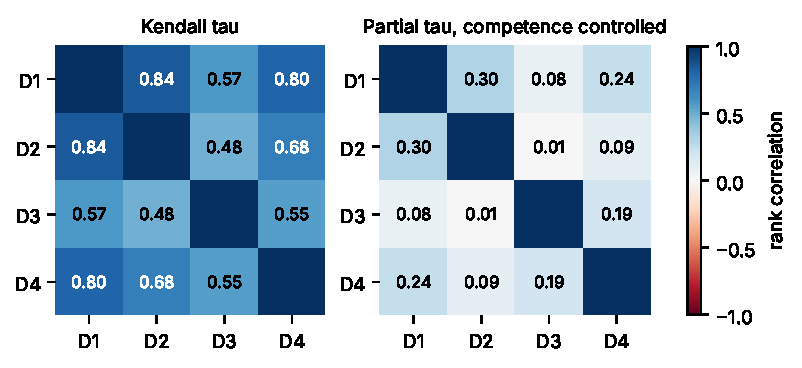
\includegraphics[width=0.85\textwidth]{othello_h1.pdf}
    \caption{Rank agreement between the diagnostics, raw (left) and with competence controlled (right).}
    \label{fig:h1}
\end{figure}

On raw scores the diagnostics agree: five of six pairs meet the agreement rule, D2 with D3 is partial, and
Kendall's W is 0.872 (Table~\ref{tab:h1}, Figure~\ref{fig:h1}). But every diagnostic follows competence: its
tau with competence is 0.968 for D1, 0.826 for D2, 0.790 for D4 and 0.577 for D3. D1 is above the 0.90 line of
rule A5, so its controlled pairs are not interpretable, and the controlled conclusion rests on the three pairs
among D2, D3 and D4. All three lose their agreement: D2 with D3 disagrees outright, and D2 with D4 and D3 with
D4 are agreement through competence. On ranks with competence removed, W falls to 0.267.

\paragraph{Sensitivity (A3).} On the 23 models with competence of at least 0.90, where tau(D1, competence) is
0.855 and A5 does not apply, three pairs still agree on raw scores (D1 with D2, D1 with D4, D2 with D4), and
after the control only D1 with D2 agrees (partial tau 0.532 [0.088, 0.838]); W is 0.830 raw and 0.466 on
residual ranks. The direction is the same as on the full zoo.

\paragraph{Answer to H1.} The four diagnostics agree on which Othello models are better, but mostly because they
all measure how competent the model is. With competence controlled, the three diagnostics that can be
separated from competence do not measure the same thing.

\subsection{Disagreement (H2)}
\label{sec:h2}

The mean disagreement per model (the standard deviation of its four rank percentiles) is 0.089, against a seed
noise floor of 0.028. By factor, the mean disagreement is 0.094, 0.087 and 0.084 for transformers, LSTMs and
Mamba; 0.110, 0.083 and 0.073 for small, medium and large models; and 0.075, 0.102 and 0.089 for synthetic,
championship and mixed training data. The F tests give $p=0.783$ for architecture, $p=0.027$ for scale (0.081
after Holm correction) and $p=0.171$ for training data (0.341 after Holm). No factor is significant after the
correction, so under the preregistered rule \textbf{the disagreement is consistent with noise}. Scale comes
closest: small models are ranked least consistently.

\subsection{Predictive validity (H3)}
\label{sec:h3}

\paragraph{The outcome first.} Relative fragility v2 has mean 0.015, standard deviation 0.070 and range
$-0.124$ to 0.215, and 52\% of the models are below 0, that is, slightly better under the shifts than on their
own test games. Most models are therefore not very fragile, and the spread H3 tries to predict is small.

\begin{table}[H]
    \centering
    \small
    \begin{tabular}{lrl}
    \toprule
    Diagnostic & Statistic [95\% CI] & Adds to D1 \\
    \midrule
    D1 (reference), Spearman with relative fragility v2 & 0.150 [$-0.315$, 0.588] & \\
    D2, partial Spearman given D1 & 0.031 [$-0.297$, 0.438] & no \\
    D3, partial Spearman given D1 & 0.026 [$-0.373$, 0.386] & no \\
    D4, partial Spearman given D1 & $-0.554$ [$-0.734$, $-0.124$] & yes \\
    \bottomrule
    \end{tabular}
    \caption{H3 on 81 models. Fragility is ``higher breaks more'', so a negative value means a higher score goes
    with less breaking.}
    \label{tab:h3}
\end{table}

D1 alone does not predict fragility. Among D2, D3 and D4, only D4 adds to D1 (Table~\ref{tab:h3}); its
regression coefficient with D1, architecture and scale is $-1.48$ [$-2.47$, $-0.60$]. D4 is the strongest, but
its difference to D2 has the interval [$-1.114$, 0.098], which includes 0, so under the preregistered rule
\textbf{no single diagnostic wins}. The result is the same without the test model ($-0.561$ [$-0.738$, $-0.117$])
and on relative fragility v1 ($-0.540$ [$-0.693$, $-0.197$]). The raw Spearman correlations of all four
diagnostics with the outcome are near 0 (0.15, 0.15, 0.13 and $-0.04$), so the D4 signal appears only after D1
is controlled. The causal label adds nothing beyond D4 selectivity (partial $-0.049$ [$-0.241$, 0.122]).

\subsection{Exploratory: where the fragility and the D4 signal come from}
\label{sec:exploratory}

The analyses in this subsection were decided after the preregistered results were read and are reported as
exploratory. The models trained on human championship games behave differently from the rest: their mean
relative fragility is $+0.090$, against $-0.024$ for synthetic and $-0.022$ for mixed training, and their mean
D4 is the lowest (0.175, against 0.236 for synthetic). Figure~\ref{fig:shifts} shows why they are fragile: they
break on random games (a mean drop of 0.190) and on rotated or reflected boards (0.14 to 0.18), while synthetic
and mixed models barely change under any shift. Human games cover a narrow part of the game tree and are
recorded in one orientation. Under forced detours every group is slightly more often legal than on its own
line, so detours do not make these models fragile.

\begin{figure}[H]
    \centering
    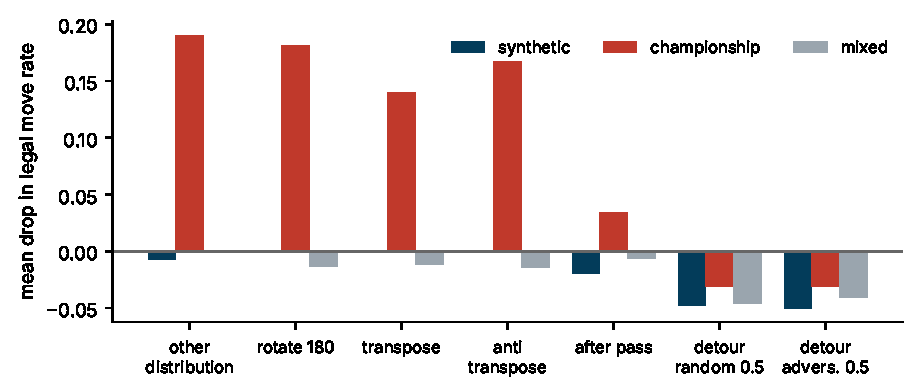
\includegraphics[width=0.95\textwidth]{othello_shifts.pdf}
    \caption{Mean drop in legal move rate per fragility v2 shift, by training distribution (exploratory).
    ``Other distribution'' averages both other distributions for mixed models.}
    \label{fig:shifts}
\end{figure}

\begin{figure}[H]
    \centering
    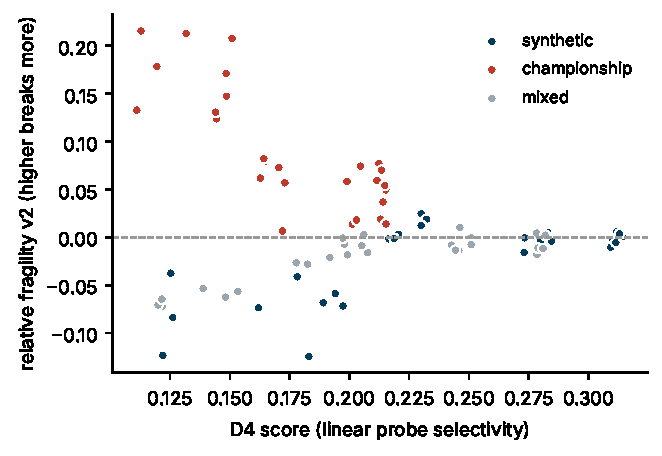
\includegraphics[width=0.6\textwidth]{othello_h3_d4.pdf}
    \caption{D4 against relative fragility v2, one point per model, by training distribution.}
    \label{fig:h3}
\end{figure}

\begin{table}[H]
    \centering
    \small
    \begin{tabular}{lr}
    \toprule
    D4 partial Spearman with relative fragility v2, given D1 & value [95\% CI] \\
    \midrule
    all 81 models (preregistered) & $-0.554$ [$-0.734$, $-0.124$] \\
    within synthetic (27 models) & $+0.449$ [$-0.226$, 0.726] \\
    within championship (27 models) & $-0.530$ [$-0.761$, 0.191] \\
    within mixed (27 models) & $+0.341$ [$-0.221$, 0.666] \\
    all 81, controlling for D1 and training distribution & $+0.231$ [$-0.336$, 0.589] \\
    \bottomrule
    \end{tabular}
    \caption{The D4 result within and across training distributions (exploratory).}
    \label{tab:simpson}
\end{table}

Within each training distribution the D4 link is not there: its sign flips between distributions and every
interval includes 0, and with training data added as a control it is $+0.231$ (Table~\ref{tab:simpson},
Figure~\ref{fig:h3}). The same holds for D2 ($+0.153$ [$-0.346$, 0.555]) and D3 ($-0.259$ [$-0.502$, 0.078]).
The preregistered D4 result is computed exactly as planned, but it is a between distribution effect, a
Simpson's paradox: it says that championship trained models are both less probe readable and more fragile,
not that probing predicts fragility among comparable models. With nine configurations per distribution the
within distribution estimates are imprecise, so the honest summary is that \textbf{no diagnostic shows a
reliable link to fragility among comparable Othello models}.

\subsection{Held out domain (H4)}
H4 is not yet tested. It requires H1 to H3 to be fixed on Othello and navigation first; the interpreter models
are then trained and scored with the same code, and the Othello answers above are the first half of what they
will be compared against.

% ------------------------------------------------------------------------------------------------------------------------
\section{Discussion}

The Othello results answer the question that motivated the project, at least for one domain. Published claims
for and against world models in Othello rely on different diagnostics, and our results suggest why they can
disagree without either being wrong in its own terms: the diagnostics share a large common factor, competence,
and beyond it they measure different things. A paper that reports one diagnostic on models of different quality
will mostly be reporting how good the models are.

What each diagnostic licenses a researcher to claim follows from this. D1 measures competence and nothing
more. D2 adds information about whether the model's predictions depend on the board rather than the move order,
but its distinction error shows that even good models often fail to separate boards with different legal moves.
D3, at the protocol we preregistered, gives small gaps on the zoo and partly rewards an occupancy shortcut that
the move list gives away. D4 shows that the board is decodable in every model, while the causal check shows
that only a few models, almost all trained on synthetic games, use it. ``Decodable'' is therefore not the same
claim as ``has a world model'', which is what Li et al.~\cite{li2023othello} and Belinkov~\cite{belinkov2022probing}
warned about.

For predictive validity, the result is a caution rather than a ranking: on Othello the fragility suite mostly
separates the championship trained models from the rest, so any diagnostic that also separates them looks
predictive. Navigation, where the three training distributions differ less sharply in coverage, is a better
test of H3, and we plan to preregister a training distribution control for it before any navigation score
exists.

\subsection{Limitations}
\begin{itemize}
    \item \textbf{One domain so far.} All results are for Othello; navigation and the held out interpreter are
    still to come, and H4 is untested.
    \item \textbf{Few independent units.} The 81 models are 27 configurations; the configuration bootstrap makes
    the intervals honest but wide, and within distribution analyses rest on nine configurations each.
    \item \textbf{D2 uses next move continuations only}, which keeps it cheap but is a simplification of Vafa et
    al.~\cite{vafa2024evaluating}, and its same board pairs come mostly from the opening.
    \item \textbf{D3 measures help from pretraining with 64 examples}, not closeness to a perfect answer, and
    part of it reflects an occupancy shortcut.
    \item \textbf{Fragility is small on most models}, so H3 rests on the minority of fragile models; version 1
    of the suite had two parts that could not measure fragility on this zoo, corrected in version 2 before
    scoring.
    \item \textbf{The mixed distribution} trains on about 85\% synthetic games, not 50\%, as described in
    Section~\ref{sec:data}.
    \item \textbf{Compute.} Every model has the same modest budget on a single A10G; the best zoo models
    (competence up to 0.969) remain below the published Othello GPT, and Mamba runs without its optimized kernels.
\end{itemize}

% ------------------------------------------------------------------------------------------------------------------------
\section{Conclusion and Future Work}

On 81 Othello models and under a preregistered analysis: \textbf{H1}, the four diagnostics agree on which models
are better, but almost entirely through competence, and the diagnostics that can be separated from competence
do not agree once it is controlled. \textbf{H2}, their disagreement is not systematic in architecture, scale or
training data. \textbf{H3}, no single diagnostic wins; D4 adds to the legal move rate, but an exploratory check
shows that this comes from differences between training distributions. \textbf{H4} is still to be tested on the
held out interpreter.

Next, the same pipeline runs on navigation, starting with a reproduction of the state equivalence results of
Vafa et al.~\cite{vafa2024evaluating}, and then on the held out interpreter for H4, with the paper due on
December 8. Beyond this project, the same comparison could be extended to domains with continuous or
probabilistic state, and any new world model diagnostic can be added through the common interface and judged
against these four on identical ground truth.

\bibliographystyle{IEEEtran}
\bibliography{references}

% ------------------------------------------------------------------------------------------------------------------------
\appendix
\section{Team Roles}

\begin{table}[H]
    \centering
    \small
    \begin{tabular}{l>{\raggedright\arraybackslash}p{10.5cm}}
    \toprule
    Member & Responsibility \\
    \midrule
    Siddardha Reddy & coordination; D4 representation probing, reproduction gate and causal check; rules engine,
    data and model interface; preregistration and amendments; scoring launcher and H1 to H3 analysis \\
    Nikhil Obuleni & zoo trainer and throughput; D3 inductive bias probe; fragility suite; continuous
    integration; Streamlit demo \\
    Viharika Vemparala & D1 next token validity; report skeleton; data and splits write up \\
    Venkatesh Nagarjuna & D2 state equivalence review and sign off; proposal and progress reports; presentation \\
    \bottomrule
    \end{tabular}
    \caption{Main responsibilities. Each member trained and scored one slice of the zoo on their own instance;
    the analysis and the paper are shared.}
\end{table}

\section{Reproducibility}

Code, data references, results and tags are in the repository
\url{https://github.com/nik-hill-323/fall-2026-group6}. From the repository root:
\begin{itemize}
    \item train one slice of the zoo (slice number 0 to 4):\\ \texttt{bash src/shellscripts/train\_slice.sh}
    \item score one slice with every diagnostic and both fragility suites:\\
    \texttt{bash src/shellscripts/score\_slice.sh}
    \item run the preregistered analysis (master table, result files and figures):\\
    \texttt{python src/analysis/hypotheses.py}
    \item run the exploratory analysis:\\ \texttt{python src/analysis/exploratory\_othello.py}
    \item make the figures of this report:\\ \texttt{python reports/Latex\_report/make\_figures.py}
\end{itemize}
A plain language summary of every Othello result is in \texttt{results/analysis/othello/RESULTS.md}.

\end{document}
